% Volume I: Mathematical Language and Finite-Dimensional Geometry
% Continuity note for Chapter 2.
% Previous dependencies: Chapter 1's typed objects, statements, sets, relations, and modeling-as-compression habit.
% New durable concepts: functions as typed maps; domain/codomain/image/preimage; injective/surjective/bijective maps; coordinates as representations; change of coordinates; data transformations; monoids, groups, and structure-preserving maps.
% Forward hooks: vectors as coordinate-bearing objects in Chapter 3; matrices as linear transformations in Chapter 4; projections and fitting in Chapter 5; PCA, manifolds, random variables, symmetries, and learned representations later.
% Notation commitments: use \(f:X\to Y\), \(f(A)\), \(f^{-1}(B)\), \([v]_B\), \(v=B[v]_B\), \(z_i=A(x_i-\mu)+b\), \(S_z=A S_x A^\top\), and \(\phi(gx)=\rho(g)\phi(x)\).
% Figure plan: four raster ImageGen figures under imagegen-figures/ch02-* cover functions/preimages, coordinate systems, data transformations, and algebraic structures.
\section{Chapter 2: Functions, Transformations, and Coordinate Systems}
\label{ch:functions-transformations-coordinate-systems}

Chapter 1 taught us to ask what kind of object a symbol names. This chapter asks the next question: once the objects are typed, how do we move between them, describe them with coordinates, and recognize structure that survives a change of description?

The central habit is to separate an object from its representation. A function is not merely a formula. It is a rule with a domain and codomain. A coordinate system is not the object itself. It is a way of naming locations with numbers. A data transformation is not cosmetic preprocessing. It changes the representation seen by an algorithm. An algebraic structure records which operations are allowed and which laws they obey. These ideas will reappear as random variables, neural encoders, embeddings, feature maps, symmetries, coordinate changes, and learned representations.

\paragraph{Chapter problem.}
How can we change descriptions without losing track of what object, data set, or structure is being described?

\paragraph{Section map.}
Section 2.1 defines functions as typed mappings and shows how output-side questions pull back to input-side sets. Section 2.2 treats coordinates as numerical descriptions of the same underlying object. Section 2.3 turns preprocessing into explicit transformations of data clouds. Section 2.4 records the algebraic laws that make transformations composable, reversible, or symmetry-respecting.

\subsection{2.1 Functions as mappings}

\paragraph{Motivating question.}
What does a function \(f:X\to Y\) actually do to individual inputs, subsets, and questions about outputs?

\paragraph{Beginner setup.}
A \emph{function} from a set \(X\) to a set \(Y\) assigns to every input \(x\in X\) exactly one output \(f(x)\in Y\). The set \(X\) is the domain. The set \(Y\) is the codomain. The domain says which inputs are legal; the codomain says what kind of output the rule promises to produce.

The smallest nontrivial example is
\[
X=\{x_1,x_2,x_3,x_4\},\qquad
Y=\{y_1,y_2,y_3\},
\]
with
\[
f(x_1)=y_1,\quad f(x_2)=y_1,\quad f(x_3)=y_2,\quad f(x_4)=y_3.
\]
This is a function even though two inputs share the same output. A function is not required to be reversible. It is required only to give one output for each allowed input.

A rule fails to be a function if it gives no output for an allowed input, or if it gives two different outputs for the same input. For example, a lookup table that sends \(x_1\) to both \(y_1\) and \(y_2\) is not a function \(X\to Y\). It may be a relation or a stochastic rule, but it is not a deterministic function until the ambiguity is resolved.

A noisy response model is still typed carefully. If a stimulus can produce several spike counts on repeated trials, the deterministic object might be the map from stimulus to a distribution over spike counts, not a map that sends one stimulus to several simultaneous outputs. That distinction keeps the function language useful without pretending biological responses are noiseless.

Functions solve the problem of controlled dependence: they let us say that an output is determined by an input. In computation, a function may be a Python routine, a neural network layer, a fitted encoding model, a coordinate chart, or a statistic computed from data. In mathematics, the same language also lets us ask how sets move. If \(A\subseteq X\), then \(f(A)\subseteq Y\) is the set of outputs reached by inputs in \(A\). If \(B\subseteq Y\), then \(f^{-1}(B)\subseteq X\) is the set of inputs whose outputs land in \(B\).

What to keep in mind: \(f^{-1}(B)\) does not require \(f\) to have an inverse function. It is a preimage of a set, not necessarily an inverse value of a point.

\begin{figure}[htbp]
\centering
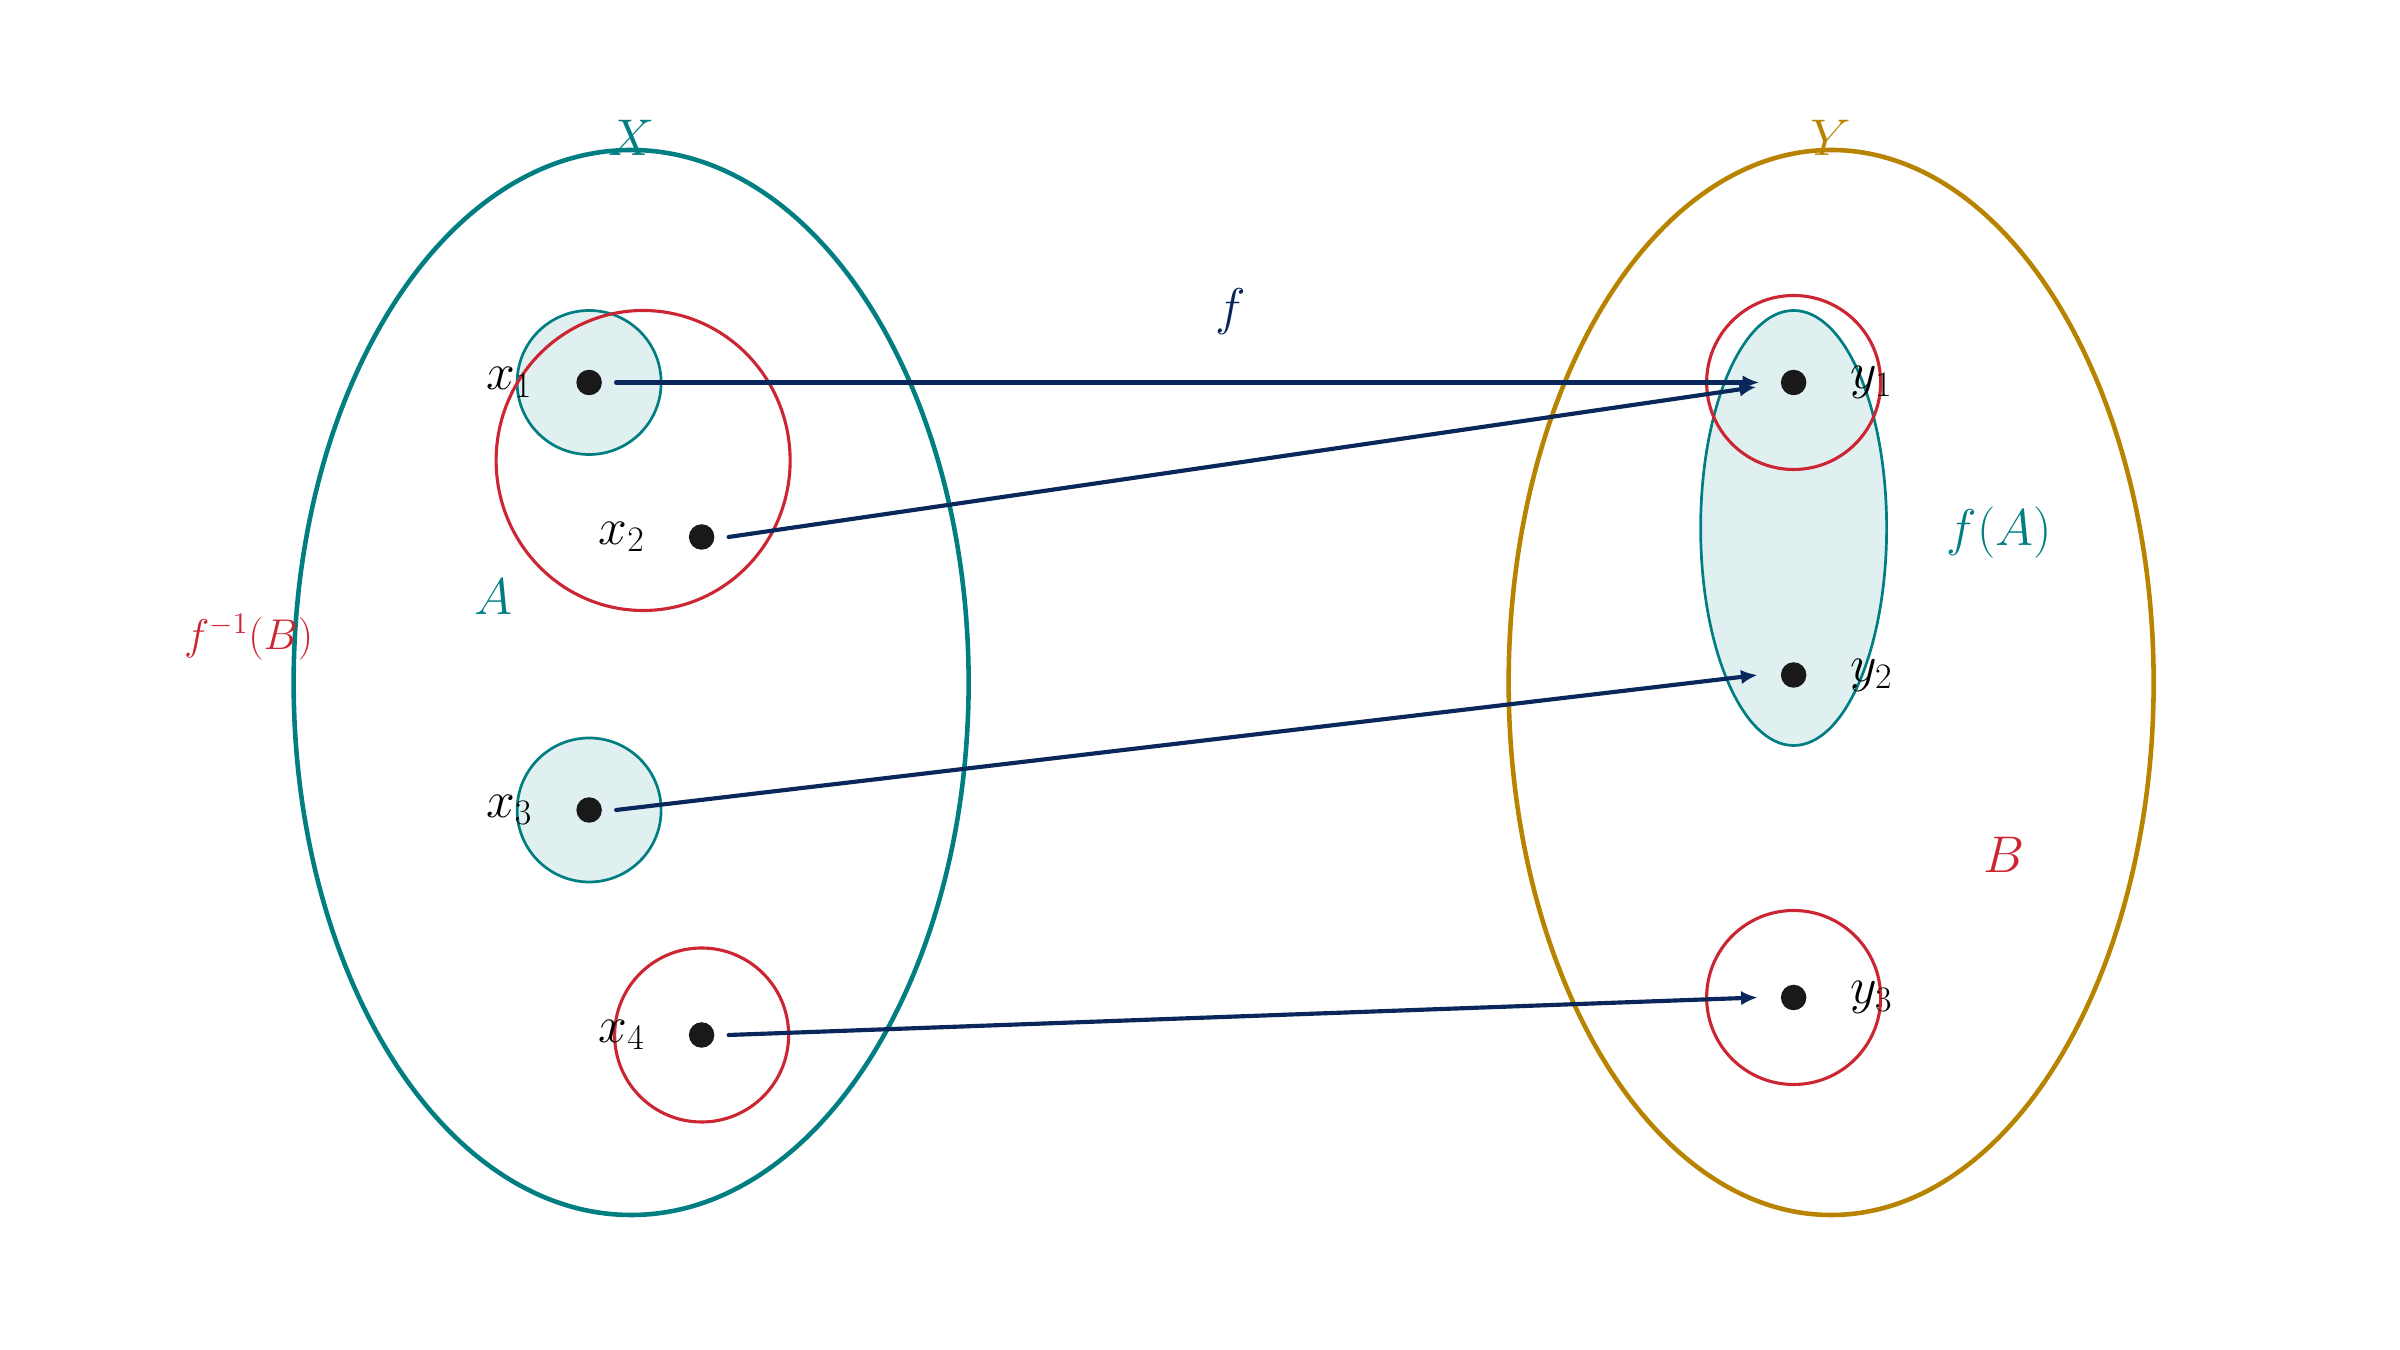
\includegraphics[width=0.92\linewidth]{imagegen-figures/ch02-functions-as-mappings.png}
\caption{A function moves points and induces set-level maps. Each \(x_i\in X\) has exactly one image in \(Y\), but several inputs may share an output. The teal region illustrates an image \(f(A)\). The red contours illustrate the preimage \(f^{-1}(B)=\{x_1,x_2,x_4\}\) of the output-side set \(B=\{y_1,y_3\}\).}
\label{fig:ch02-functions-as-mappings}
\end{figure}

\paragraph{Formal setup.}
Let \(X\) and \(Y\) be sets. A function \(f:X\to Y\) is a rule such that for every \(x\in X\), there exists a unique \(y\in Y\) with \(y=f(x)\). For \(A\subseteq X\), the \emph{image} of \(A\) is
\[
f(A)=\{f(x):x\in A\}\subseteq Y.
\]
For \(B\subseteq Y\), the \emph{preimage} of \(B\) is
\[
f^{-1}(B)=\{x\in X:f(x)\in B\}\subseteq X.
\]
The full image \(f(X)\) is also called the range. The function is \emph{injective} if \(f(x)=f(x')\) implies \(x=x'\). It is \emph{surjective} if \(f(X)=Y\). It is \emph{bijective} if it is both injective and surjective; only then does it have an inverse function \(f^{-1}:Y\to X\).

If \(f:X\to Y\) and \(g:Y\to Z\), their \emph{composition} is the function
\[
g\circ f:X\to Z,\qquad (g\circ f)(x)=g(f(x)).
\]
The codomain of \(f\) must match the domain of \(g\). This type check is what makes a chain of maps mathematically legal.

For a finite output set \(Y\), a stochastic response model can be written as a deterministic function
\[
K:X\to \Delta(Y),
\]
where \(\Delta(Y)\) is the set of probability distributions on \(Y\). The sampled output may vary from trial to trial, but the model object \(K\) still has a domain, codomain, and well-defined value at each input.

\paragraph{Core intuition.}
The useful picture is not a graph of \(y=f(x)\) on axes, but a mapping diagram: points in the domain flow to points in the codomain. Figure~\ref{fig:ch02-functions-as-mappings} shows two kinds of movement. Images push input-side sets forward. Preimages pull output-side questions backward. If \(B\) means ``the model predicts class 1,'' then \(f^{-1}(B)\) is the set of inputs classified as class 1. If \(B\) means ``spike count at least 5,'' then \(f^{-1}(B)\) is the set of stimuli that evoke that response category.

Common misconceptions are easy to diagnose. First, a formula without a domain and codomain is not yet a fully specified function. The formula \(x^2\) defines different functions on \(\mathbb{R}\), on \(\mathbb{R}_{\ge 0}\), and on a finite data set. Second, the point preimage \(f^{-1}(\{y\})\) may contain several points or none at all unless \(f\) is bijective. Third, the codomain \(Y\) may be larger than the actual image \(f(X)\); unused labels are still allowed outputs by type, but not produced by this particular function.

This section extends Chapter 1's typed-object discipline. Later, preimages become the way random variables turn events in value-space into events in outcome-space. Images become reachable states in dynamics. Level sets \(f^{-1}(\{c\})\) become decision boundaries, iso-response curves, and constraint surfaces.

\paragraph{Main theorem: preimages preserve logical operations.}
For any function \(f:X\to Y\) and any subsets \(B,C\subseteq Y\),
\[
f^{-1}(B\cup C)=f^{-1}(B)\cup f^{-1}(C),
\]
\[
f^{-1}(B\cap C)=f^{-1}(B)\cap f^{-1}(C),
\]
and
\[
f^{-1}(Y\setminus B)=X\setminus f^{-1}(B).
\]

\emph{Proof sketch.} We prove the union identity by checking membership. An input \(x\in X\) belongs to \(f^{-1}(B\cup C)\) exactly when \(f(x)\in B\cup C\). That means \(f(x)\in B\) or \(f(x)\in C\). Translating each condition back to \(X\), this says \(x\in f^{-1}(B)\) or \(x\in f^{-1}(C)\). That is exactly membership in \(f^{-1}(B)\cup f^{-1}(C)\).

The intersection proof is the same with ``or'' replaced by ``and.'' For the complement identity, \(x\in f^{-1}(Y\setminus B)\) exactly when \(f(x)\notin B\), which exactly means \(x\notin f^{-1}(B)\). The mechanism is important: preimages preserve the logic of output-side questions because they translate a statement about \(f(x)\) into a statement about \(x\).

\paragraph{Worked examples.}
\emph{Small numerical example.} Let \(X=\{1,2,3,4,5\}\), \(Y=\{0,1,2\}\), and let \(f(x)\) be the remainder of \(x\) after division by \(3\). Then
\[
f(1)=1,\quad f(2)=2,\quad f(3)=0,\quad f(4)=1,\quad f(5)=2.
\]
If \(A=\{1,2,3\}\), then \(f(A)=\{0,1,2\}\). If \(B=\{1,2\}\), then
\[
f^{-1}(B)=\{1,2,4,5\}.
\]
The preimage is larger than \(B\) because it lives in a different set: it is a subset of inputs, not a subset of outputs.

If \(g:Y\to\{\text{even},\text{odd}\}\) labels \(0\) and \(2\) as even and \(1\) as odd, then \((g\circ f)(5)=g(2)=\text{even}\). Composition means the output type of the first map becomes the input type of the next.

\emph{Conceptual ML/neuroscience example.} Let \(f_\theta:X\to\{0,1\}\) be a binary classifier that maps an image to a decision. The set \(f_\theta^{-1}(\{1\})\) is the decision region for class \(1\). In neuroscience, let \(r:S\to\mathbb{R}_{\ge 0}\) map a stimulus \(s\) to a predicted firing rate. The preimage \(r^{-1}([20,\infty))\) is the set of stimuli predicted to drive the neuron above \(20\) spikes per second. In both cases, the important object is a region in input space defined by an output-side condition.

\paragraph{ML/DL/neuroscience connections.}
In supervised learning, \(f_\theta\) maps inputs to predictions, while a loss \(\ell(f_\theta(x),y)\) maps predictions and targets to numbers. In deep learning, a network is a composition of functions whose intermediate codomains are activation spaces. In probability, a random variable is a function \(X:\Omega\to\mathbb{R}\); events such as \(\{X>0\}\) are preimages of subsets of \(\mathbb{R}\). In neural encoding, a tuning curve is a function from stimulus variables to response summaries, and its level sets describe stimuli treated equivalently by the neuron.

\paragraph{Exercises.}
\begin{enumerate}[label=\textbf{2.1.\arabic*.}, leftmargin=*]
\item \textbf{Mechanical.} Let \(f:\{a,b,c,d\}\to\{0,1,2\}\) be given by \(f(a)=0\), \(f(b)=1\), \(f(c)=1\), and \(f(d)=2\). Compute \(f(\{a,c\})\), \(f^{-1}(\{1\})\), and \(f^{-1}(\{0,2\})\).
\item \textbf{Proof or derivation.} Prove that \(f(A\cup C)=f(A)\cup f(C)\) for \(A,C\subseteq X\). Then give an example showing that \(f(A\cap C)=f(A)\cap f(C)\) can fail.
\item \textbf{Numerical/computational.} Write pseudocode that, given a finite dictionary representing \(f:X\to Y\) and a subset \(B\subseteq Y\), returns \(f^{-1}(B)\).
\item \textbf{Interpretation.} A classifier outputs three labels: rest, reach, and grasp. What input-side set is represented by \(f^{-1}(\{\text{reach},\text{grasp}\})\)?
\item \textbf{Debug the misconception.} A student says, ``Since \(f^{-1}(\{y\})\) is written with an inverse symbol, \(f\) must be invertible.'' Explain why this is false and state what \(f^{-1}(\{y\})\) means.
\end{enumerate}

\subsection{2.2 Coordinate systems and representations}

\paragraph{Motivating question.}
When the same point has coordinates \((3,2)\) in one system and \((1,2)\) in another, what has changed and what has stayed the same?

\paragraph{Beginner setup.}
A \emph{coordinate system} assigns numbers to geometric or abstract objects so that we can compute with them. The object is the point, vector, state, or stimulus. The coordinates are its numerical description relative to a chosen reference system.

The smallest nontrivial example is a point \(p\) in the plane. In the usual horizontal-vertical axes, it may have coordinates \([p]_E=(3,2)\). In a tilted basis \(B=(b_1,b_2)\), the same point may be described as \([p]_B=(1,2)\), meaning one step along \(b_1\) plus two steps along \(b_2\). The point did not move. The measuring frame changed.

Coordinate systems solve the problem of computation. Geometry is coordinate-free, but algorithms need arrays of numbers. A neural population state, an image, a word embedding, or a latent variable may be the same mathematical object viewed through different coordinate choices.

What to keep in mind: coordinates are names, not the object itself. A coordinate change should change the numbers while preserving the underlying point and any coordinate-independent facts about it.

\begin{figure}[htbp]
\centering
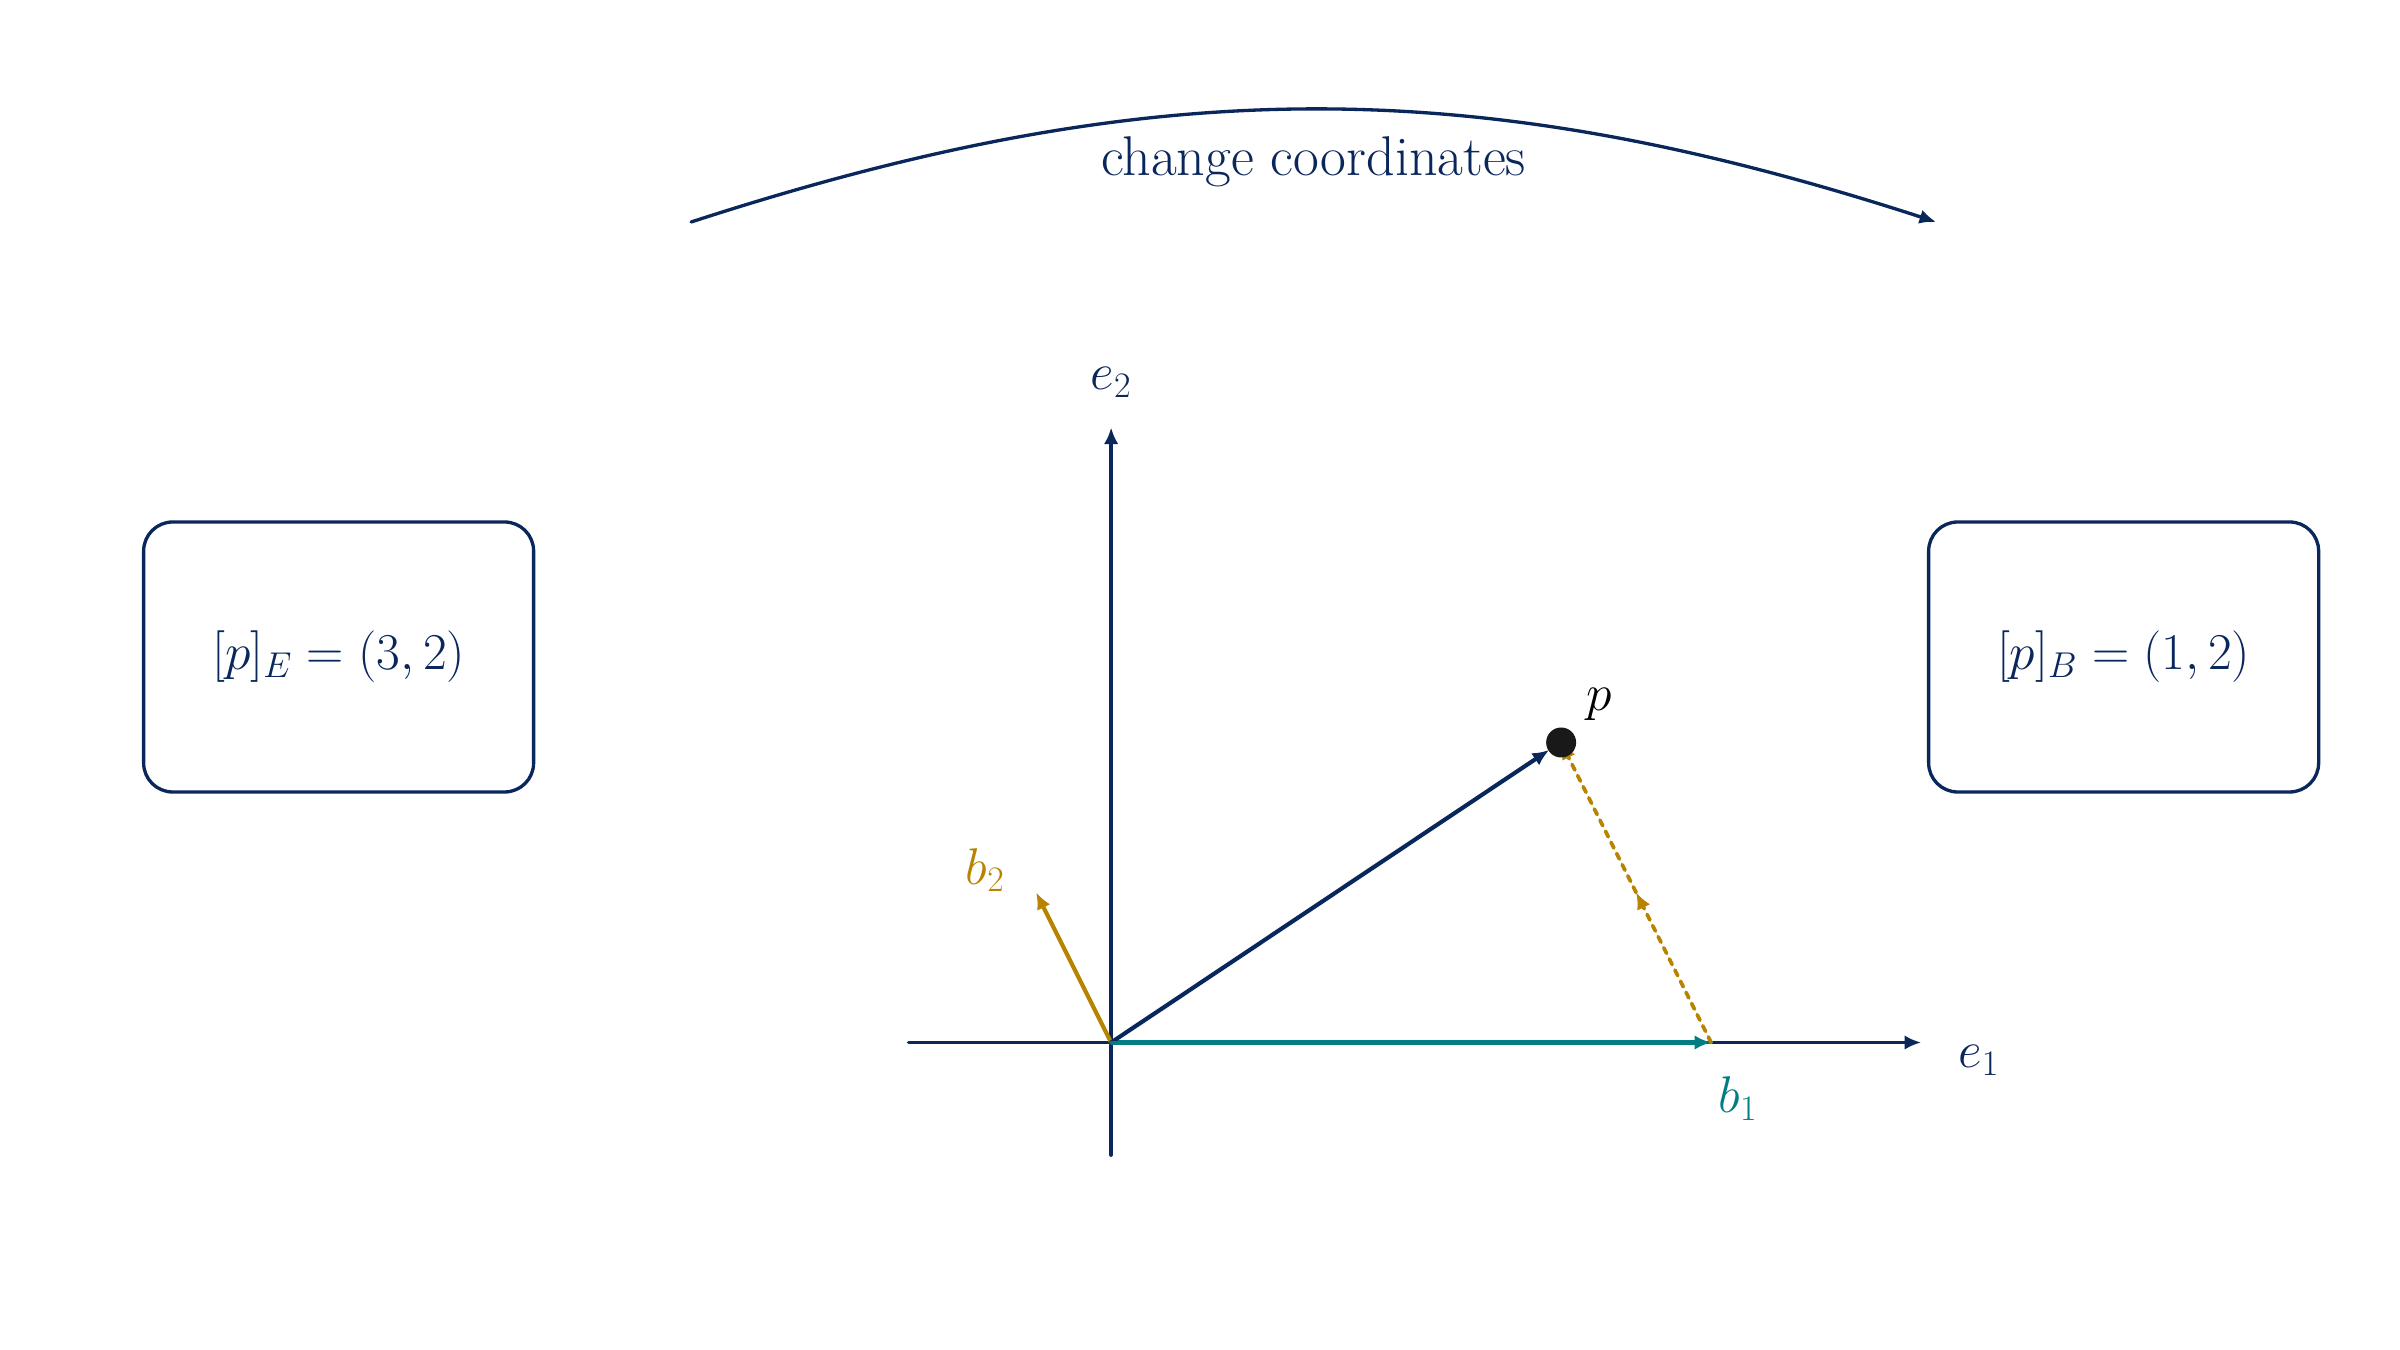
\includegraphics[width=0.92\linewidth]{imagegen-figures/ch02-coordinate-systems.png}
\caption{One point, two coordinate descriptions. The dot \(p\) is fixed in the plane. The standard axes \(e_1,e_2\) give \([p]_E=(3,2)\), while one \(b_1\) step and two \(b_2\) steps give \([p]_B=(1,2)\). The change-of-coordinates arrow changes the numerical representation, not the geometric point.}
\label{fig:ch02-coordinate-systems}
\end{figure}

\paragraph{Formal setup.}
Work in \(\mathbb{R}^n\). A basis \(B=(b_1,\dots,b_n)\) is an ordered list of \(n\) vectors such that every vector \(v\in\mathbb{R}^n\) can be written uniquely as
\[
v=a_1b_1+\cdots+a_nb_n.
\]
The coordinate vector of \(v\) in basis \(B\) is
\[
[v]_B=\begin{bmatrix}a_1\\ \vdots\\ a_n\end{bmatrix}.
\]
If the basis vectors are placed as columns of a matrix, also denoted \(B\), then the object-level vector and its coordinates satisfy
\[
v=B[v]_B.
\]
Equivalently, the coordinate map for basis \(B\) is
\[
\kappa_B:\mathbb{R}^n\to\mathbb{R}^n,\qquad \kappa_B(v)=[v]_B,
\]
with inverse reconstruction map \(\kappa_B^{-1}(a)=Ba\). The same set \(\mathbb{R}^n\) appears on both sides, but the meanings differ: one side is the ambient object, and the other is a list of coefficients relative to \(B\).
For another basis \(C=(c_1,\dots,c_n)\),
\[
v=C[v]_C.
\]
The dimensions matter: \(B\) and \(C\) are \(n\times n\) invertible matrices; \([v]_B\) and \([v]_C\) are column vectors in \(\mathbb{R}^n\); \(v\) is the underlying vector in the ambient space.

More generally, a representation map
\[
r:\mathcal{O}\to R\subseteq\mathbb{R}^k
\]
assigns coordinate-like arrays to objects in some object space \(\mathcal{O}\). A basis coordinate system on \(\mathbb{R}^n\) is reversible, because \(v\) can be reconstructed from \([v]_B\). A learned representation or summary statistic may be nonreversible: two different objects can share the same representation if the representation intentionally discards details.

\paragraph{Core intuition.}
Think of a coordinate system as a measuring grid laid over the same space. Standard coordinates count horizontal and vertical steps. A tilted basis counts tilted steps. Figure~\ref{fig:ch02-coordinate-systems} shows dashed coordinate steps reaching the same point \(p\). The coordinates are different because the unit directions are different.

The most common misconception is to treat a coordinate vector as if it were the object without remembering the basis. The column \(\begin{bmatrix}1\\2\end{bmatrix}\) does not by itself say where the point is; it says ``one of the first coordinate direction and two of the second,'' after a coordinate system has been specified. A second misconception is that changing coordinates changes the data-generating system. Often it changes only our description. A third is to think all coordinates are equally convenient. They are equivalent in principle, but very unequal computationally: the right coordinates can reveal low-dimensional structure, sparsity, independence, or symmetry.

This section looks backward to functions because a coordinate system is itself a map from objects to numbers. It looks forward to linear algebra, PCA, manifolds, latent variable models, embeddings, and neural population geometry.

\paragraph{Main derivation: change of coordinates.}
If \(B\) and \(C\) are two bases of \(\mathbb{R}^n\), then
\[
[v]_C=C^{-1}B[v]_B.
\]

\emph{Derivation.} Start with the same object written in two coordinate systems:
\[
v=B[v]_B
\qquad\text{and}\qquad
v=C[v]_C.
\]
Because both right-hand sides equal the same vector \(v\), we have
\[
C[v]_C=B[v]_B.
\]
The matrix \(C\) is invertible because its columns form a basis. Multiplying both sides by \(C^{-1}\) gives
\[
[v]_C=C^{-1}B[v]_B.
\]
The product \(C^{-1}B\) is the change-of-coordinates matrix from \(B\)-coordinates to \(C\)-coordinates. The algebra is short, but the interpretation is the point: reconstruct the object from its old coordinates, then remeasure it in the new basis.

\paragraph{Worked examples.}
\emph{Small numerical example.} Let \(p=(3,2)\) in standard coordinates. Choose
\[
b_1=\begin{bmatrix}4\\0\end{bmatrix},\qquad
b_2=\begin{bmatrix}-1/2\\1\end{bmatrix}.
\]
Then
\[
1b_1+2b_2=
\begin{bmatrix}4\\0\end{bmatrix}
+2\begin{bmatrix}-1/2\\1\end{bmatrix}
=\begin{bmatrix}3\\2\end{bmatrix}.
\]
So \([p]_E=(3,2)\) but \([p]_B=(1,2)\). The two columns describe the same point using different measuring directions.

\emph{Conceptual ML/neuroscience example.} A trial in a neural population experiment can be represented as a vector \(v\in\mathbb{R}^n\), where coordinate \(i\) is neuron \(i\)'s firing rate. That is the neuron basis. After dimensionality reduction, the same trial may be represented by coordinates along latent axes: movement direction, preparatory state, or a low-dimensional neural mode. The object is the trial state; the representation changes from neuron coordinates to latent coordinates.

\paragraph{ML/DL/neuroscience connections.}
In deep learning, an embedding is a coordinate representation of an input in a learned feature space. In transformers, token embeddings, residual stream coordinates, and attention-head bases are different ways of representing activations. In neuroscience, population activity can be described in neuron coordinates, principal-component coordinates, factor-analysis coordinates, or task-variable coordinates. Later, PCA will choose coordinates that align with high-variance directions; manifolds will use local coordinates; and information geometry will compare coordinate systems on spaces of probability distributions.

\paragraph{Exercises.}
\begin{enumerate}[label=\textbf{2.2.\arabic*.}, leftmargin=*]
\item \textbf{Mechanical.} Let \(b_1=(1,1)\) and \(b_2=(1,-1)\). Compute the standard-coordinate vector \(v\) with \([v]_B=(3,2)\).
\item \textbf{Proof or derivation.} Starting from \(v=B[v]_B=C[v]_C\), derive the formula for \([v]_B\) in terms of \([v]_C\).
\item \textbf{Numerical/computational.} For \(B=\begin{bmatrix}1&1\\0&1\end{bmatrix}\) and \(v=(4,3)\), solve \(B[v]_B=v\) for \([v]_B\).
\item \textbf{Interpretation.} In a neural population with \(100\) neurons, what is the difference between neuron coordinates and a three-dimensional latent coordinate system fitted to the same trials?
\item \textbf{Debug the misconception.} A student says, ``The vector \((1,2)\) is smaller than \((3,2)\), so the point moved closer to the origin after changing coordinates.'' Explain what information is missing from that comparison.
\end{enumerate}

\subsection{2.3 Transformations of data}

\paragraph{Motivating question.}
When we center, scale, rotate, embed, or otherwise preprocess data, what mathematical map has been applied and what structure does it change?

\paragraph{Beginner setup.}
A \emph{data transformation} is a function applied to observations before analysis or learning. If observations are \(x_1,\dots,x_n\in\mathbb{R}^d\), a transformation \(T:\mathbb{R}^d\to\mathbb{R}^k\) produces transformed observations
\[
z_i=T(x_i)\in\mathbb{R}^k.
\]
The output dimension \(k\) may equal \(d\), be smaller, or be larger.

The smallest nontrivial example is standardizing one feature. If \(x=(2,4,6)\), the mean is \(\mu=4\), and the scale is \(\sigma=2\), then
\[
z_i=\frac{x_i-\mu}{\sigma}
\]
gives \((-1,0,1)\). The data values changed, but in a controlled way: the center became \(0\), and the scale became one unit.

Transformations solve several problems. They put features on comparable scales, remove nuisance offsets, expose useful geometry, build nonlinear features, and make invariances explicit. A transformation can also destroy information, so it should always be named and typed.

What to keep in mind: preprocessing is mathematics. Every centering, normalization, embedding, convolution, or pooling operation is a map with consequences for distances, variances, neighborhoods, and learnability.

\begin{figure}[htbp]
\centering
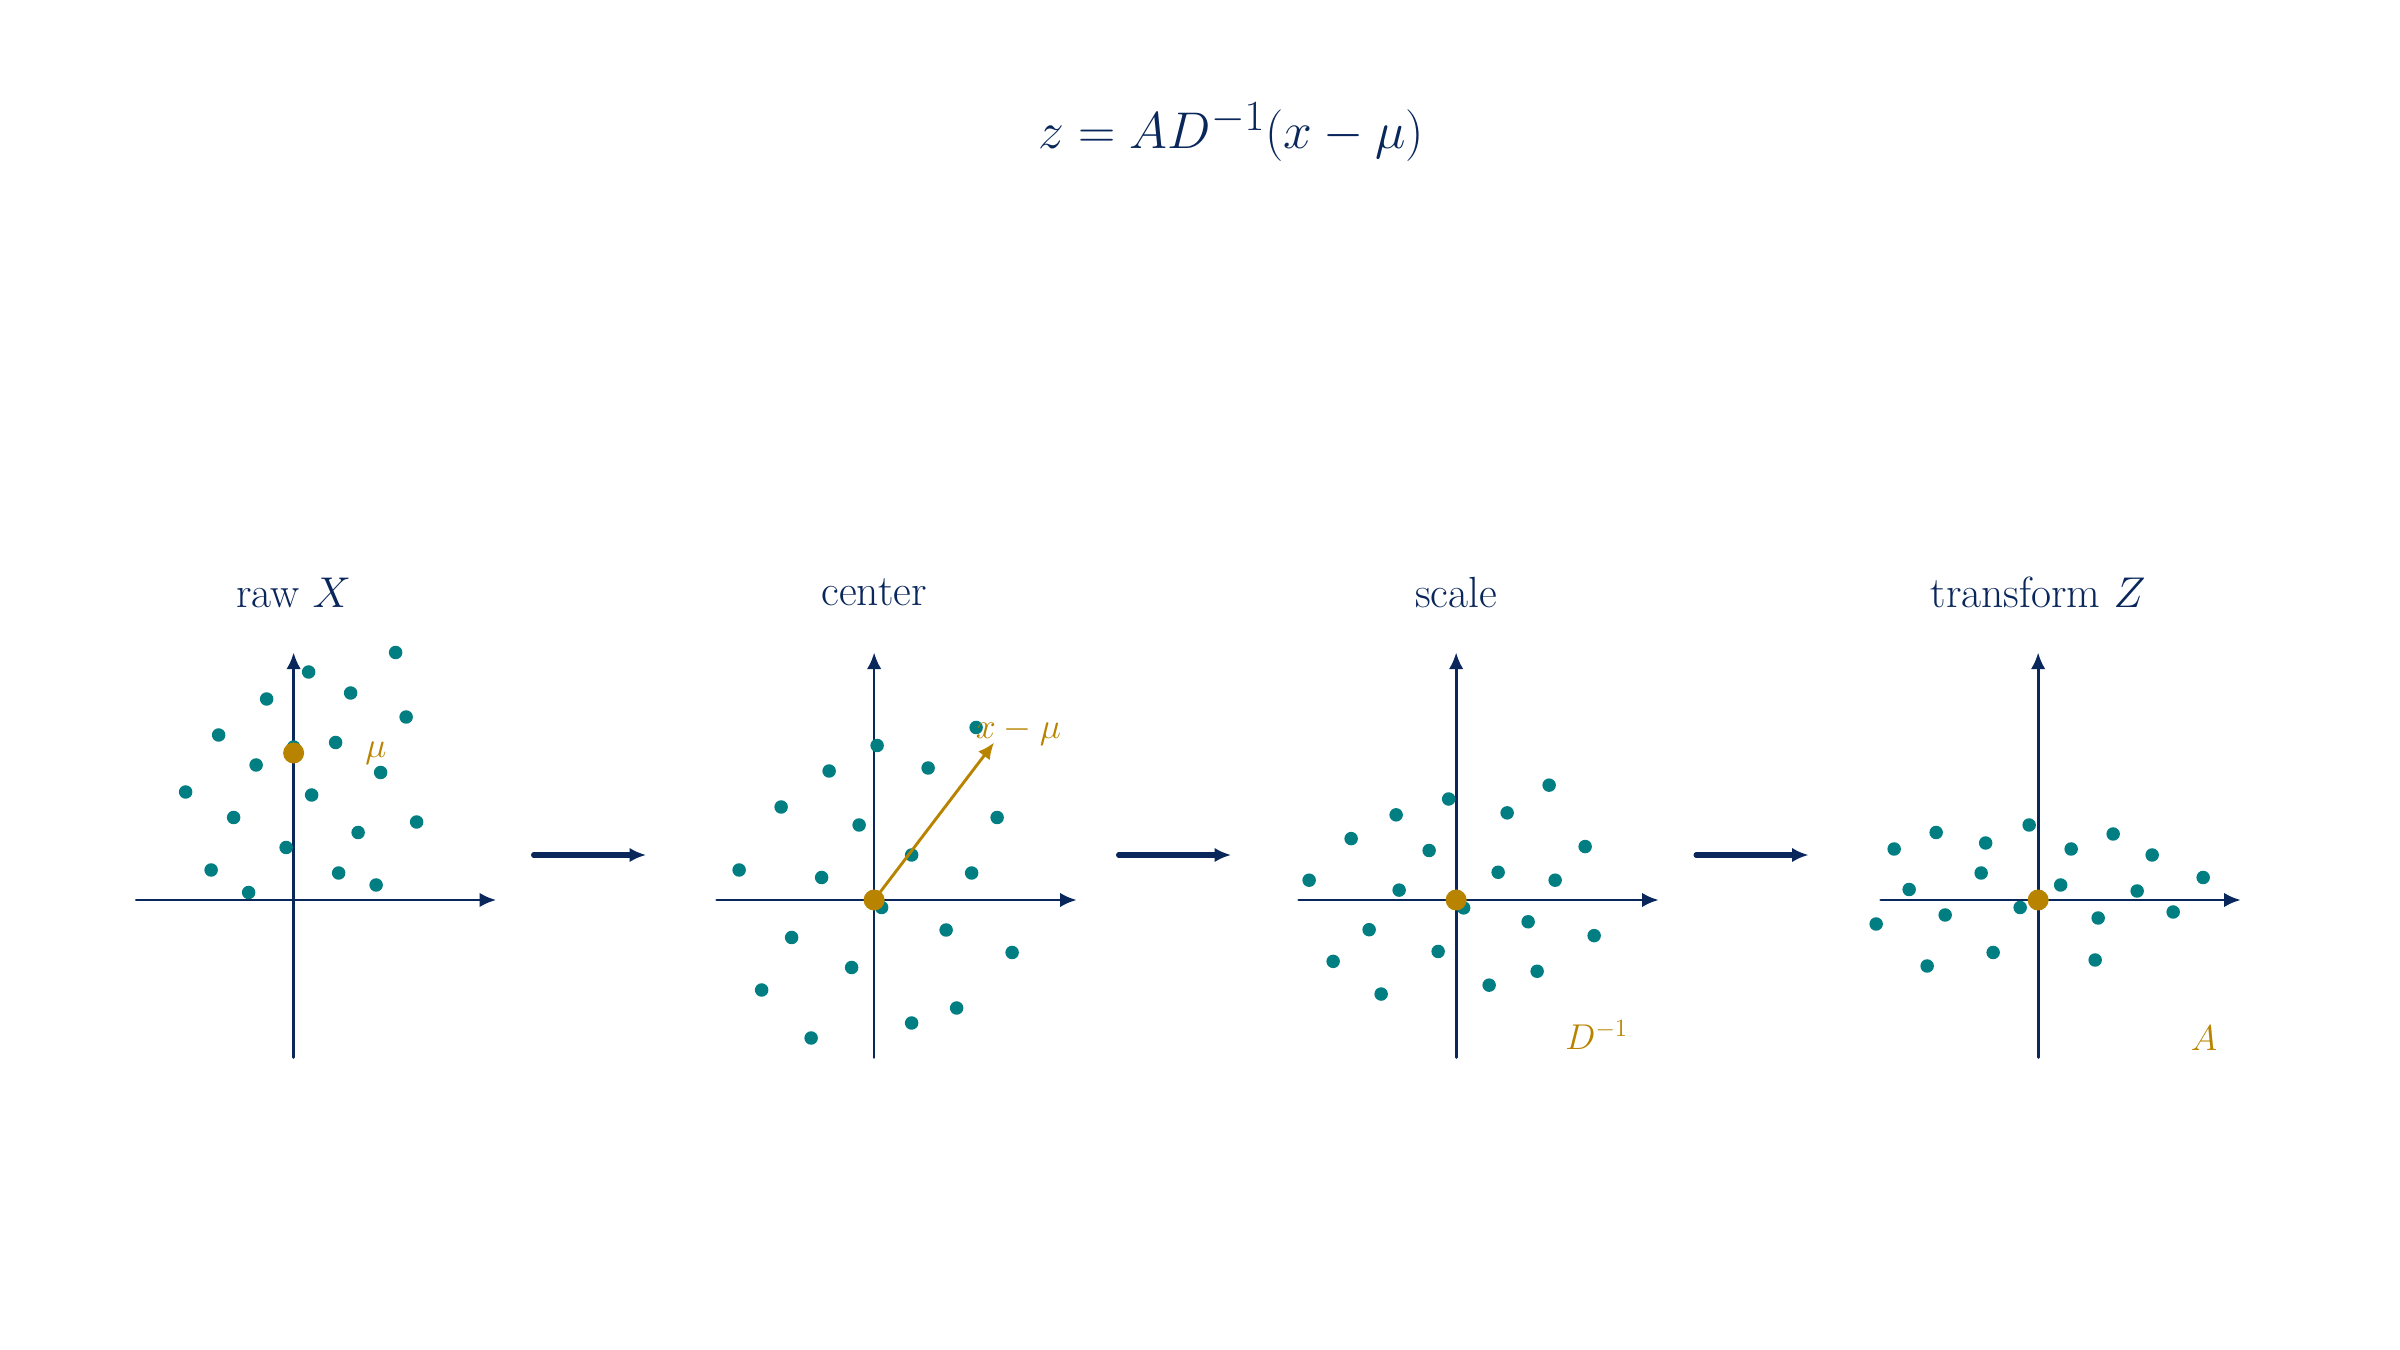
\includegraphics[width=0.95\linewidth]{imagegen-figures/ch02-data-transformations.png}
\caption{A data transformation as a pipeline of explicit maps. The raw cloud is centered by subtracting \(\mu\), scaled by \(D^{-1}\), and then transformed by \(A\) into a representation \(Z\). Each step changes a different geometric feature: location, units, and orientation.}
\label{fig:ch02-data-transformations}
\end{figure}

\paragraph{Formal setup.}
Let \(x_1,\dots,x_n\in\mathbb{R}^d\) be data points. The empirical mean is
\[
\bar x=\frac{1}{n}\sum_{i=1}^n x_i.
\]
The empirical covariance matrix is
\[
S_x=\frac{1}{n}\sum_{i=1}^n (x_i-\bar x)(x_i-\bar x)^\top.
\]
Consider an affine-linear transformation
\[
z_i=A(x_i-\mu)+b,
\]
where \(A\in\mathbb{R}^{k\times d}\), \(\mu\in\mathbb{R}^d\), and \(b\in\mathbb{R}^k\). A common preprocessing special case is
\[
z_i=A D^{-1}(x_i-\mu),
\]
where \(D=\operatorname{diag}(\sigma_1,\dots,\sigma_d)\) rescales coordinates before applying \(A\). The inverse \(D^{-1}\) is defined only when every scale entry satisfies \(\sigma_j\ne 0\); in standard preprocessing these scale entries are usually positive.

Not every useful data transformation is affine. A nonlinear feature map
\[
\phi:\mathbb{R}^d\to\mathbb{R}^k,\qquad x\mapsto \phi(x)
\]
might add coordinates such as \(x_1^2\), \(x_1x_2\), thresholded features, or learned hidden activations. The same typing questions remain: what is the input space, what is the output space, and which information can be recovered from the transformed representation?

The recovery question is a function question from Section 2.1. A transformation \(T:\mathbb{R}^d\to\mathbb{R}^k\) is information-preserving on a data set if distinct data points remain distinct after applying \(T\). It is lossy on that data set if two different points \(x_i\ne x_j\) satisfy \(T(x_i)=T(x_j)\). Lossy transformations are often useful, but they must be interpreted as summaries rather than neutral rewritings.

\paragraph{Core intuition.}
Data transformations move an entire point cloud. Centering changes location. Scaling changes units and relative spreads. Rotation or projection changes the axes used to describe variation. A nonlinear feature map may unfold a curved pattern or make a classifier possible. Figure~\ref{fig:ch02-data-transformations} shows a point cloud passing through centering, scaling, and a final transformation.

Common misconceptions: standardization does not make data Gaussian; rotation does not change pairwise distances if it is an orthogonal rotation, but projection can; and a representation with more dimensions is not automatically more informative if the added coordinates are deterministic copies or noise. Invertible transformations preserve recoverability of the original point, while many-to-one transformations such as pooling, thresholding, or projection usually discard information. Another frequent mistake is to transform training data and test data using different fitted parameters. If \(\mu\) and \(D\) are estimated from training data, those same values must be used at test time.

This section depends on functions and coordinates. A transformation is a function; a useful transformation often chooses a more convenient coordinate representation. Later, gradients will transform errors backward, PCA will transform data into variance-aligned coordinates, kernels will transform data implicitly, and neural networks will learn transformations layer by layer.

\paragraph{Main derivation: mean and covariance under an affine map.}
For \(z_i=A(x_i-\mu)+b\),
\[
\bar z=A(\bar x-\mu)+b
\]
and
\[
S_z=A S_x A^\top.
\]

\emph{Derivation.} Average the transformed data:
\[
\bar z=\frac{1}{n}\sum_{i=1}^n \bigl(A(x_i-\mu)+b\bigr).
\]
Linearity of matrix multiplication lets \(A\) pass outside the sum, and \(b\) appears \(n\) times:
\[
\bar z=A\left(\frac{1}{n}\sum_{i=1}^n x_i-\mu\right)+b
=A(\bar x-\mu)+b.
\]
Now subtract the transformed mean:
\[
z_i-\bar z
=A(x_i-\mu)+b-\bigl(A(\bar x-\mu)+b\bigr)
=A(x_i-\bar x).
\]
The offset \(\mu\) and translation \(b\) cancel in the centered data. Therefore
\[
S_z=\frac{1}{n}\sum_{i=1}^n (z_i-\bar z)(z_i-\bar z)^\top
=\frac{1}{n}\sum_{i=1}^n A(x_i-\bar x)(x_i-\bar x)^\top A^\top
=A S_x A^\top.
\]
The lesson is geometric: translations move the cloud but do not change its covariance; linear maps reshape covariance.

\paragraph{Worked examples.}
\emph{Small numerical example.} For one-dimensional data \(x=(2,4,6)\), let \(\mu=4\) and \(\sigma=2\). The standardized values are
\[
z=\left(\frac{2-4}{2},\frac{4-4}{2},\frac{6-4}{2}\right)=(-1,0,1).
\]
The transformed mean is \(0\). The transformation has made the feature unitless relative to the chosen scale.

\emph{Conceptual ML/neuroscience example.} In neural population analysis, each trial may be a vector \(x_i\in\mathbb{R}^d\) of firing rates. Subtracting \(\mu\) removes baseline firing. Scaling can prevent high-rate neurons from dominating low-rate neurons. A matrix \(A\) can project the population into latent coordinates that emphasize task-related variation. The covariance formula \(S_z=A S_x A^\top\) says exactly how trial-to-trial variability changes under that projection.

\paragraph{ML/DL/neuroscience connections.}
In ML pipelines, normalization maps raw features into numerically stable coordinates for optimization. In convolutional networks, each layer transforms an image representation into feature maps; pooling then transforms local activity into coarser summaries. In contrastive learning, augmentations are transformations of inputs used to teach invariance. In neuroscience, spike counts may be square-root transformed, z-scored, smoothed, projected, or embedded; each operation changes what downstream models can see.

\paragraph{Exercises.}
\begin{enumerate}[label=\textbf{2.3.\arabic*.}, leftmargin=*]
\item \textbf{Mechanical.} Standardize the data \(x=(10,14,18)\) using \(\mu=14\) and \(\sigma=4\).
\item \textbf{Proof or derivation.} Show that adding a constant vector \(b\) to every data point changes the mean by \(b\) but leaves the covariance unchanged.
\item \textbf{Numerical/computational.} Given two-dimensional points \((1,0)\), \((3,0)\), and \((5,0)\), compute the transformed points under \(A=\begin{bmatrix}0&1\\1&0\end{bmatrix}\) and describe the geometry.
\item \textbf{Interpretation.} In a neural data set, why might subtracting each neuron's baseline firing rate help reveal task-dependent activity?
\item \textbf{Debug the misconception.} A student fits a mean and standard deviation separately on the test set before evaluating a classifier. Explain why this changes the meaning of the learned input transformation.
\end{enumerate}

\subsection{2.4 Algebraic structures}

\paragraph{Motivating question.}
How can we record not just a set of objects, but the operations that can be performed on them and the laws those operations obey?

\paragraph{Beginner setup.}
An \emph{algebraic structure} is a set together with one or more operations satisfying specified rules. The set tells us what objects exist. The operation tells us how to combine or transform them. The rules tell us which manipulations are legitimate.

The smallest nontrivial example is the integers with addition, \((\mathbb{Z},+)\). Adding two integers gives another integer. There is an identity element \(0\), because \(a+0=a\). Every integer \(a\) has an inverse \(-a\), because \(a+(-a)=0\). Addition is associative, because \((a+b)+c=a+(b+c)\). These facts are not decoration; they explain why algebraic rearrangements with integers are reliable.

Algebraic structures solve the problem of reusable reasoning. Once we know that an operation is associative, we can compose many transformations without worrying about parentheses. Once we know that inverses exist, we can undo transformations. Once we know that a symmetry group acts on data, we can define invariance and equivariance precisely.

What to keep in mind: algebra is the study of operations and laws. In this chapter, the most important algebraic objects are transformations that can be composed.

\begin{figure}[htbp]
\centering
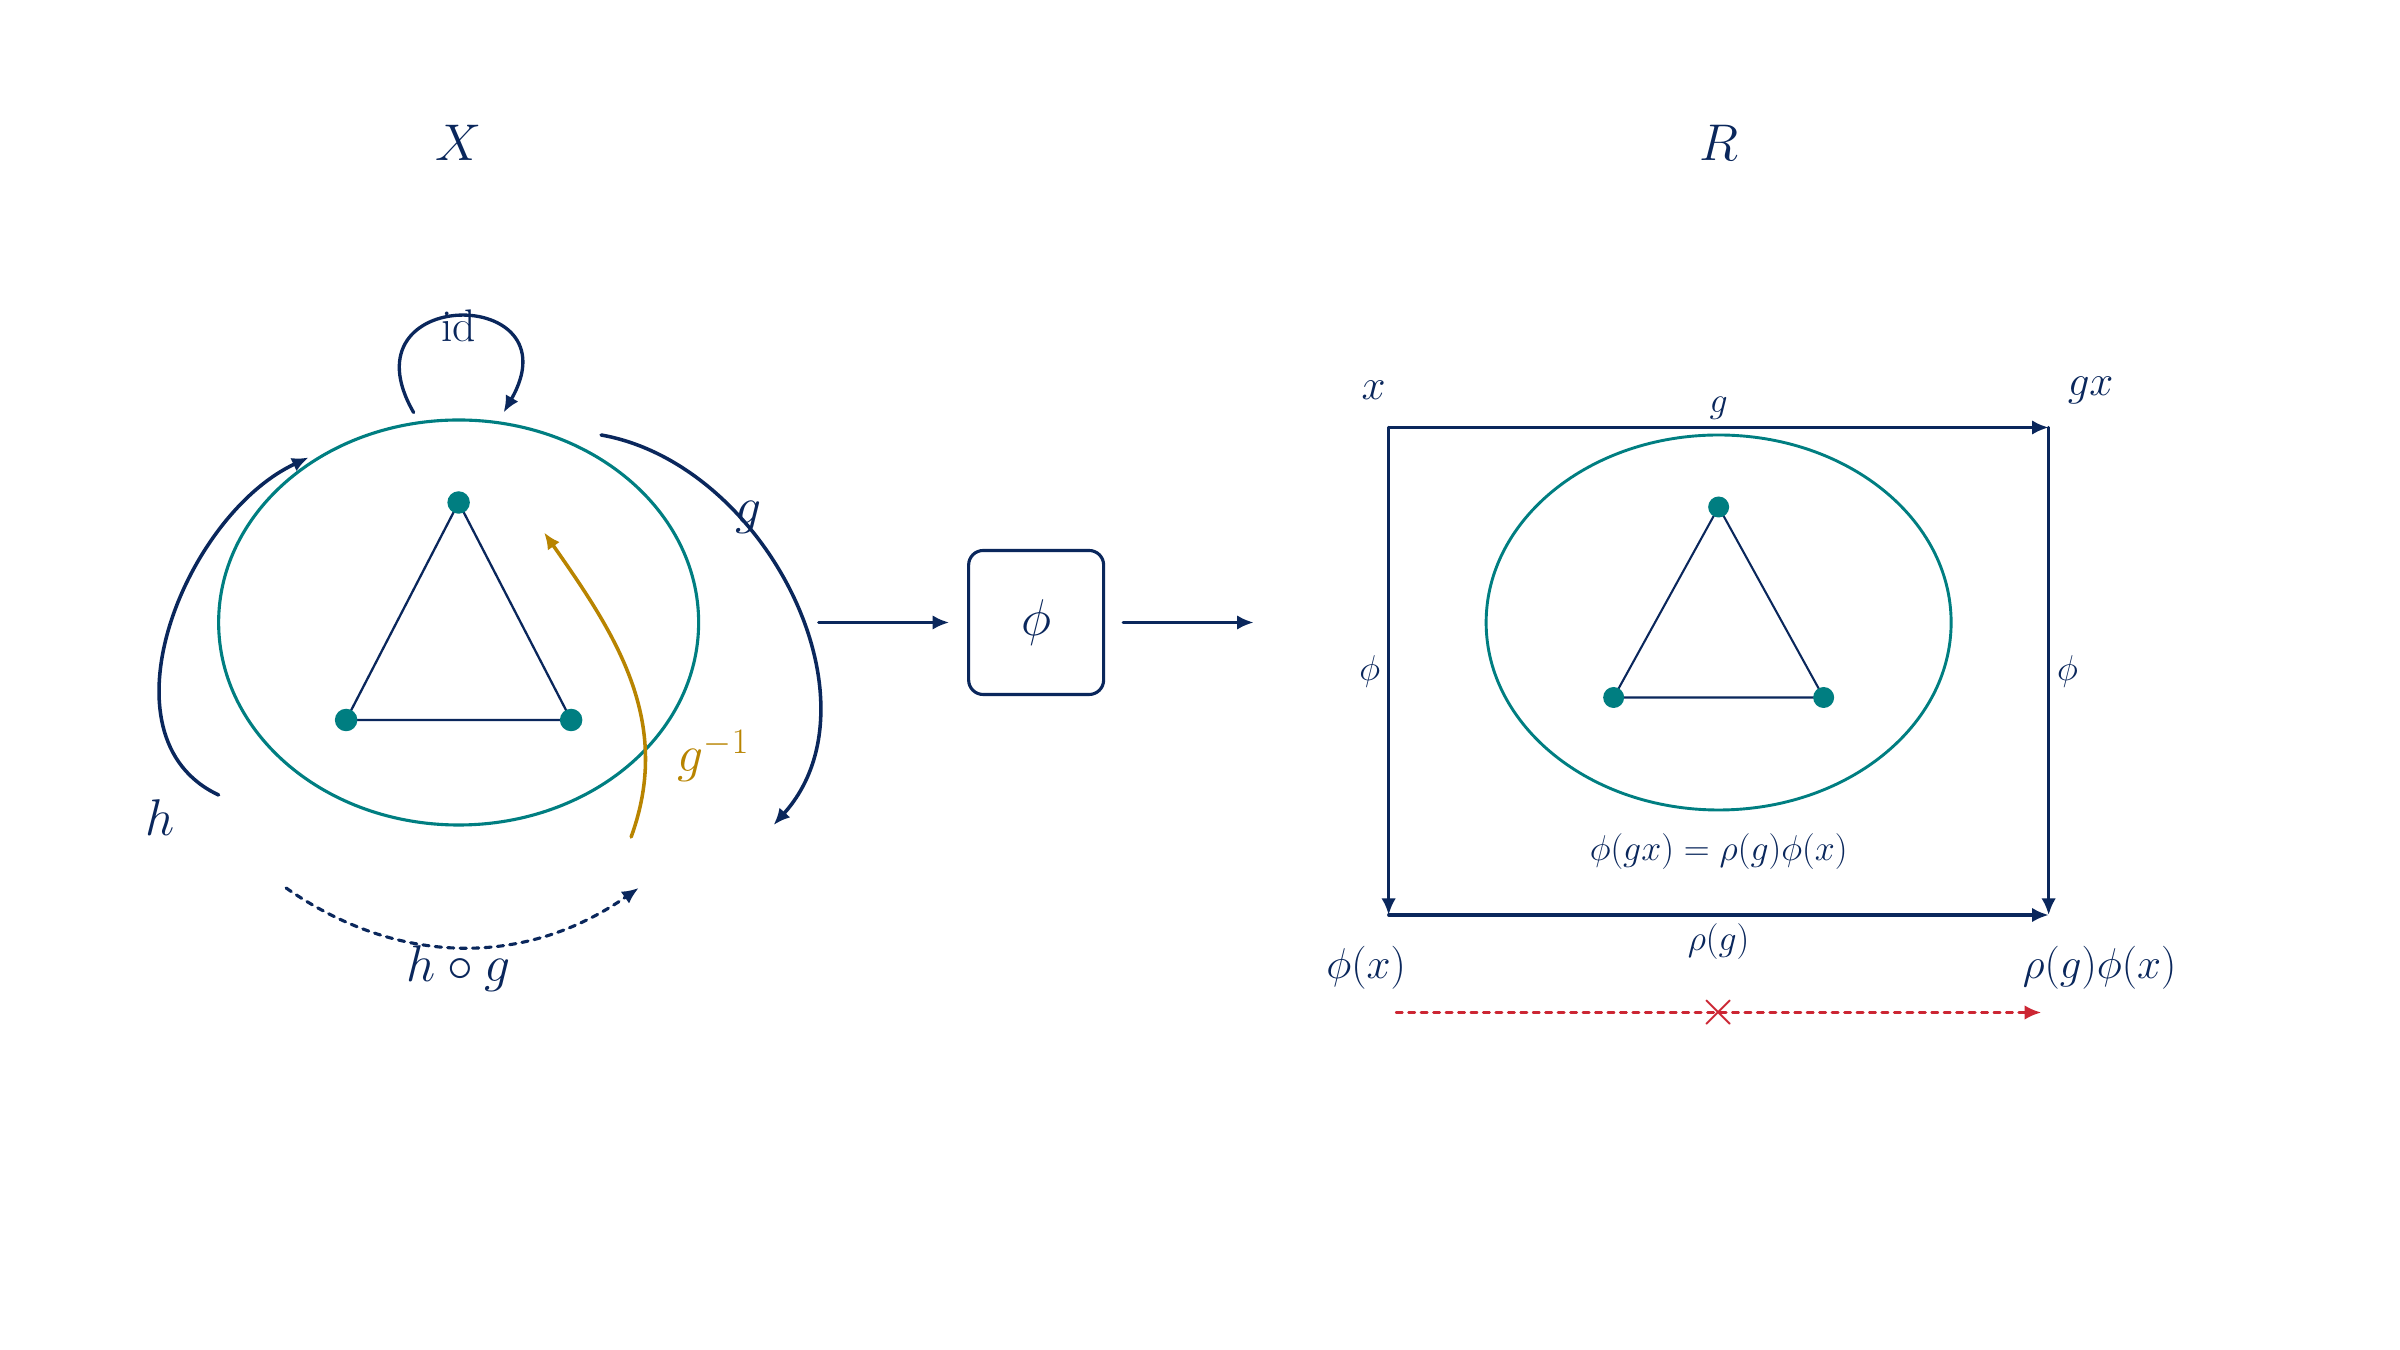
\includegraphics[width=0.95\linewidth]{imagegen-figures/ch02-algebraic-structures.png}
\caption{Algebraic structure as lawful transformation. On the left, transformations of \(X\) can be composed, have an identity action, and may have inverses. On the right, an equivariant representation \(\phi\) respects the action: transforming the input by \(g\) and then representing it matches representing it first and applying the corresponding representation-space action \(\rho(g)\).}
\label{fig:ch02-algebraic-structures}
\end{figure}

\paragraph{Formal setup.}
A binary operation on a set \(S\) is a function
\[
\star:S\times S\to S.
\]
The pair \((S,\star)\) is closed under \(\star\) by definition: combining two elements of \(S\) produces another element of \(S\). A \emph{semigroup} is a set with an associative operation:
\[
(a\star b)\star c=a\star(b\star c).
\]
A \emph{monoid} is a semigroup with an identity element \(e\in S\) such that
\[
e\star a=a\star e=a.
\]
A \emph{group} is a monoid in which every \(a\in S\) has an inverse \(a^{-1}\in S\) satisfying
\[
a^{-1}\star a=a\star a^{-1}=e.
\]
For transformations of a set \(X\), the operation is usually composition. If \(g:X\to X\) and \(h:X\to X\), their product is \(h\circ g\), meaning apply \(g\) first and then \(h\).

A map between algebraic structures should preserve the relevant operation. If \((S,\star)\) and \((T,\diamond)\) are structures, a structure-preserving map \(\phi:S\to T\) satisfies
\[
\phi(a\star b)=\phi(a)\diamond \phi(b).
\]
Equivariance is this same idea for transformations of data: applying a transformation before representation agrees with applying the corresponding transformation after representation.

Formally, suppose a group \(G\) acts on a data space \(X\), and suppose each \(g\in G\) also has a representation-space action \(\rho(g):R\to R\). A representation \(\phi:X\to R\) is equivariant when
\[
\phi(gx)=\rho(g)\phi(x)
\]
for every \(g\in G\) and \(x\in X\). It is invariant when the representation-space action is trivial, so \(\phi(gx)=\phi(x)\).

\paragraph{Core intuition.}
An algebraic structure is a rulebook for motion. The objects may be numbers, matrices, permutations, rotations, functions, or neural network layers. The operation says how motions combine. Associativity says that a chain of motions has an unambiguous result. An identity does nothing. An inverse undoes. Figure~\ref{fig:ch02-algebraic-structures} shows this idea both as composition of transformations on \(X\) and as an equivariance law transported into a representation space.

Common misconceptions: closure is not automatic for an arbitrary operation; subtraction is not associative; and a collection of transformations is not necessarily a group unless it contains identities, compositions, and inverses. Another misconception is to think algebra is detached from data. In modern ML, symmetries are algebraic assumptions about which transformations should preserve or predictably alter a representation.

This section builds on functions as mappings because transformations are functions from a set to itself. It builds on coordinate systems because the same algebraic operation can have different coordinate representations. It points forward to matrices, group equivariant networks, convolution, dynamical systems, graph symmetries, and representation geometry.

\paragraph{Main theorem: self-maps form a monoid, bijections form a group.}
Let \(X\) be a set. The set of all functions \(X\to X\), with operation given by composition, is a monoid. The subset of bijections \(X\to X\), with the same operation, is a group.

\emph{Proof sketch.} First consider all self-maps \(f:X\to X\). If \(f:X\to X\) and \(g:X\to X\), then \(g\circ f:X\to X\), so the operation is closed. Composition is associative because for every \(x\in X\),
\[
((h\circ g)\circ f)(x)=h(g(f(x)))=(h\circ(g\circ f))(x).
\]
The identity function \(\operatorname{id}_X(x)=x\) satisfies
\[
f\circ \operatorname{id}_X=f
\qquad\text{and}\qquad
\operatorname{id}_X\circ f=f.
\]
Thus all self-maps form a monoid.

Now restrict to bijections. The composition of two bijections is a bijection, so closure remains true. The identity is bijective. Every bijection \(f:X\to X\) has an inverse function \(f^{-1}:X\to X\), and
\[
f^{-1}\circ f=\operatorname{id}_X,\qquad
f\circ f^{-1}=\operatorname{id}_X.
\]
Therefore bijections form a group. The mechanism is simple but powerful: reversible transformations are exactly the transformations with algebraic inverses under composition.

\paragraph{Worked examples.}
\emph{Small symbolic example.} Let \(X=\{1,2,3\}\). Define \(g\) by \(1\mapsto2\), \(2\mapsto3\), \(3\mapsto1\), and define \(h\) by swapping \(1\) and \(2\) while leaving \(3\) fixed. Both are bijections. To compute \(h\circ g\), apply \(g\) first:
\[
1\xrightarrow{g}2\xrightarrow{h}1,\quad
2\xrightarrow{g}3\xrightarrow{h}3,\quad
3\xrightarrow{g}1\xrightarrow{h}2.
\]
So \(h\circ g\) fixes \(1\) and swaps \(2\) and \(3\). The order matters: generally \(h\circ g\ne g\circ h\).

\emph{Conceptual ML/neuroscience example.} Let \(G\) be the group of planar rotations acting on images. A representation \(\phi\) is invariant if \(\phi(gx)=\phi(x)\): rotating the image does not change the representation. It is equivariant if
\[
\phi(gx)=\rho(g)\phi(x),
\]
where \(\rho(g)\) is the corresponding transformation in representation space. In neuroscience, a population code for head direction may be equivariant to rotations: rotating the animal's heading shifts the activity bump in a predictable way rather than leaving it unchanged.

\paragraph{ML/DL/neuroscience connections.}
Convolution uses the algebra of translations: shifting an input shifts feature maps in a predictable way. Graph neural networks use permutation symmetry: relabeling nodes should not change graph-level predictions, and node-level predictions should relabel consistently. Recurrent neural networks and dynamical systems compose the same state-update map over time. In neuroscience, symmetries appear in orientation tuning, grid-cell translations, head-direction rotations, and population manifolds. Algebraic structure tells us which transformations should be ignored, inverted, or represented explicitly.

\paragraph{Exercises.}
\begin{enumerate}[label=\textbf{2.4.\arabic*.}, leftmargin=*]
\item \textbf{Mechanical.} For integers, check whether subtraction is associative by comparing \((5-3)-1\) with \(5-(3-1)\).
\item \textbf{Proof or derivation.} Prove that if \(f:X\to X\) is bijective, then its inverse function is unique.
\item \textbf{Numerical/computational.} Represent the permutation \(g=(1\ 2\ 3)\) and the swap \(h=(1\ 2)\) as dictionaries. Compute both \(h\circ g\) and \(g\circ h\).
\item \textbf{Interpretation.} In an image model, what does it mean for a representation to be invariant to translations? What information might such invariance discard?
\item \textbf{Debug the misconception.} A student says, ``Any set of data augmentations is a group.'' Identify which group laws might fail for random crops, color jitter, or additive noise.
\end{enumerate}

\paragraph{Closing bridge.}
The chapter began with typed mappings and ended with laws for composing transformations. Chapter 3 reuses both ideas in a more geometric setting. A vector will be an object with coordinates; vector addition and scalar multiplication will be algebraic operations; and later matrices will become functions that transform one coordinate-bearing object into another. The object-versus-representation distinction introduced here is the safeguard that keeps those later computations meaningful.

\clearpage
